\documentclass[grey]{beamer}
\usetheme{Warsaw}
\usepackage{graphicx}
\usepackage{color}
\usepackage{amsmath,amsthm}
\usepackage{bm}
\usepackage{amsbsy}
\usepackage{amssymb,mathrsfs,enumerate}
\usepackage{fancybox}
\usepackage{amsfonts}
\usepackage{rotating}
\usepackage{multirow}
\usepackage{epstopdf}
\usepackage{subcaption}
\usepackage{color, colortbl}
\usepackage{booktabs}
\definecolor{Gray}{gray}{0.95}

\usepackage{latexsym,amsfonts,epsfig,color,url,amssymb}
\def\qed{\quad \vrule height7.5pt width4.17pt depth0pt} 
\def\Real{{{\rm I\!R}}}
\newcommand{\Eps}{\mathcal{E}}
\newcommand{\bb}{\bf}
\newcommand{\bd}{\bm{d}}
\newcommand{\comment}[1]{}     % comment{}
\newcommand{\curl}{\mathop{\bf curl  }}
\newcommand{\grad}{\mathop{\bf grad }}
\newcommand{\Curl}{\mathop{\rm curl }}
\renewcommand{\div}{\mathop{\sf div  }}
\newcommand{\hcurl}{H(\mathbf{curl})}
\newcommand{\hCurl}{H(\Curl)}
\newcommand{\Tau}{\mathcal{T}}
\newcommand{\vCurl}{V(\Curl)}
\newcommand{\hDiv}{H(\div)}
\newcommand{\hdiv}{H(\div)}
\newcommand{\fvec}{\mathbf{f}}
\newcommand{\uvec}{\mathbf{u}}
\newcommand{\vvec}{\mathbf{v}}
\newcommand{\psvec}{\mathbf{\psi}}
\newcommand{\pvec}{\mathbf{\phi}}
\newcommand{\diag}{\mathsf{diag}}
\newcommand{\R}{{\sf R\hspace*{-0.9ex}\rule{0.15ex}{1.5ex}\hspace*{0.9ex}}}
\newcommand{\N}{{\sf N\hspace*{-1.0ex}\rule{0.15ex}{1.3ex}\hspace*{1.0ex}}}
%\newcommand{\Q}{{\sf Q\hspace*{-1.1ex}\rule{0.15ex}{1.5ex}\hspace*{1.1ex}}}
\newcommand{\Q}{\mathbb{Q}}
\newcommand{\C}{{\sf C\hspace*{-0.9ex}\rule{0.15ex}{1.3ex}\hspace*{0.9ex}}}
\newcommand{\bevs}{\vspace{-7mm}\[}
\newcommand{\eevs}{\]\vspace{-10mm}}
\newcommand{\eels}{\]\vspace{-1mm}}
\newcommand{\BA}{\begin{eqnarray}}
\newcommand{\EA}{\end{eqnarray}}
\newcommand{\BE}{\begin{equation}}
\newcommand{\EE}{\end{equation}}
\newcommand{\ba}{\begin{array}}
\newcommand{\ea}{\end{array}}
\newcommand{\baa}{\begin{eqnarray*}}
\newcommand{\eaa}{\end{eqnarray*}}
\newcommand{\be}{\begin{equation}}
\newcommand{\ee}{\end{equation}}
\newcommand{\bx}{\bm{x}}
\newcommand{\bw}{\bm{w}}
\newcommand{\bv}{\bm{v}}
\newcommand{\balpha}{\bm{\alpha}}
\newcommand{\bn}{\bm{n}}
\newcommand{\Hgr}{H^1_0(\Omega)}
\newcommand{\twopartdef}[4] {
	\left\{
		\begin{array}{ll}
			#1 & #2 \\
			#3 & #4
		\end{array}
	\right. }
\def\rot{\text{\rm rot}}

\def\Pin{{\Pi^i_{\scriptsize{n}}}}
\def\Pie{{\Pi^{h_i}}}
\def\Lti{{L^2(\Omega_i)}}

\def\Wgrad{{W^{h_i}_{\scriptsize{\mbox{grad}}}}}
\def\Wcurl{{W^{h_i}_{\scriptsize{\mbox{curl}}}}}

\def\Rtilde{{\widetilde{R}}}
\def\Stilde{{\widetilde{S}}}
\def\Wtilde{{\widetilde{W}}}
\def\Shat{{\widehat{S}}}
\def\What{{\widehat{W}}}
\def\range{{\rm \bf range} }

\newcommand{\sg}{\sigma}
\newcommand{\set}[1]{\{\,#1\,\}}    %% set notation
\uselanguage{spanish}
\languagepath{spanish}
\deftranslation[to=spanish]{Theorem}{Teorema}
\deftranslation[to=spanish]{theorem}{teorema}
\deftranslation[to=spanish]{definition}{definición}
\deftranslation[to=spanish]{Definition}{Definición}
\deftranslation[to=spanish]{example}{ejemplo}
\deftranslation[to=spanish]{Example}{Ejemplo}
\newcommand{\bN}{\mathbb{N}}
\newcommand{\bF}{\mathbb{F}}
\newcommand{\bP}{\mathbb{P}}
\newcommand{\id}{\text{id}}
\newcommand{\ord}{\text{ord}}
\newcommand{\inv}{\text{inv}}
\newcommand{\des}{\text{des}}
\newcommand{\maj}{\text{maj}}
\newcommand{\word}[1]{\quad\text{#1}\quad} %% texto intercalado

\title[Coloquio: $q$-análogos]{Explorando estadísticas de permutaciones: contando con $q$'s}
\author[I. Rojas]{\bf Ignacio Rojas \thanks{Colorado State University}}
\date{Mayo, 2023}

\begin{document}
\maketitle

%\begin{frame}{Outline}
%\begin{itemize}
%\item Introduction\\
%\item Domain Decomposition Methods\\
%\item Virtual Element Methods\\
%\item Numerical Experiments \\
%\end{itemize}
%\end{frame}

\begin{frame}[t]\frametitle{Permutaciones}
\begin{definition}
Una \underline{permutación} de un conjunto $A$ es una biyección $\sg:A\to A$.
\end{definition}\pause

Estamos más familiarizados con permutaciones de $[n]$ donde 
$$[n]=\set{1,2,\dots,n}$$\pause

\begin{itemize}
  \item Consideremos la permutación $\sg$:
  $$\sg(1)=3,\quad\sg(2)=5,\quad\sg(3)=4,\quad\sg(4)=1,\quad\sg(5)=2.$$
  Esta notación es \emph{poco conveniente}\dots
\end{itemize}

\end{frame}

\begin{frame}[t]\frametitle{Notación}
Escribamos $\sg$ de distintas formas:\pause
\begin{itemize}[<+->]
  \item Como un emparejamiento:\vspace{3em}
  \item Como una matriz:\vspace{3em}
  \item Como una lista:\vspace{3em}
  \item Como un gráfico:
\end{itemize}

\end{frame}
  
\begin{frame}[t]\frametitle{Una forma más, por ciclos:}
Tenemos $\sg=35412$:\pause
\begin{center}
  \begin{figure}
    \centering
   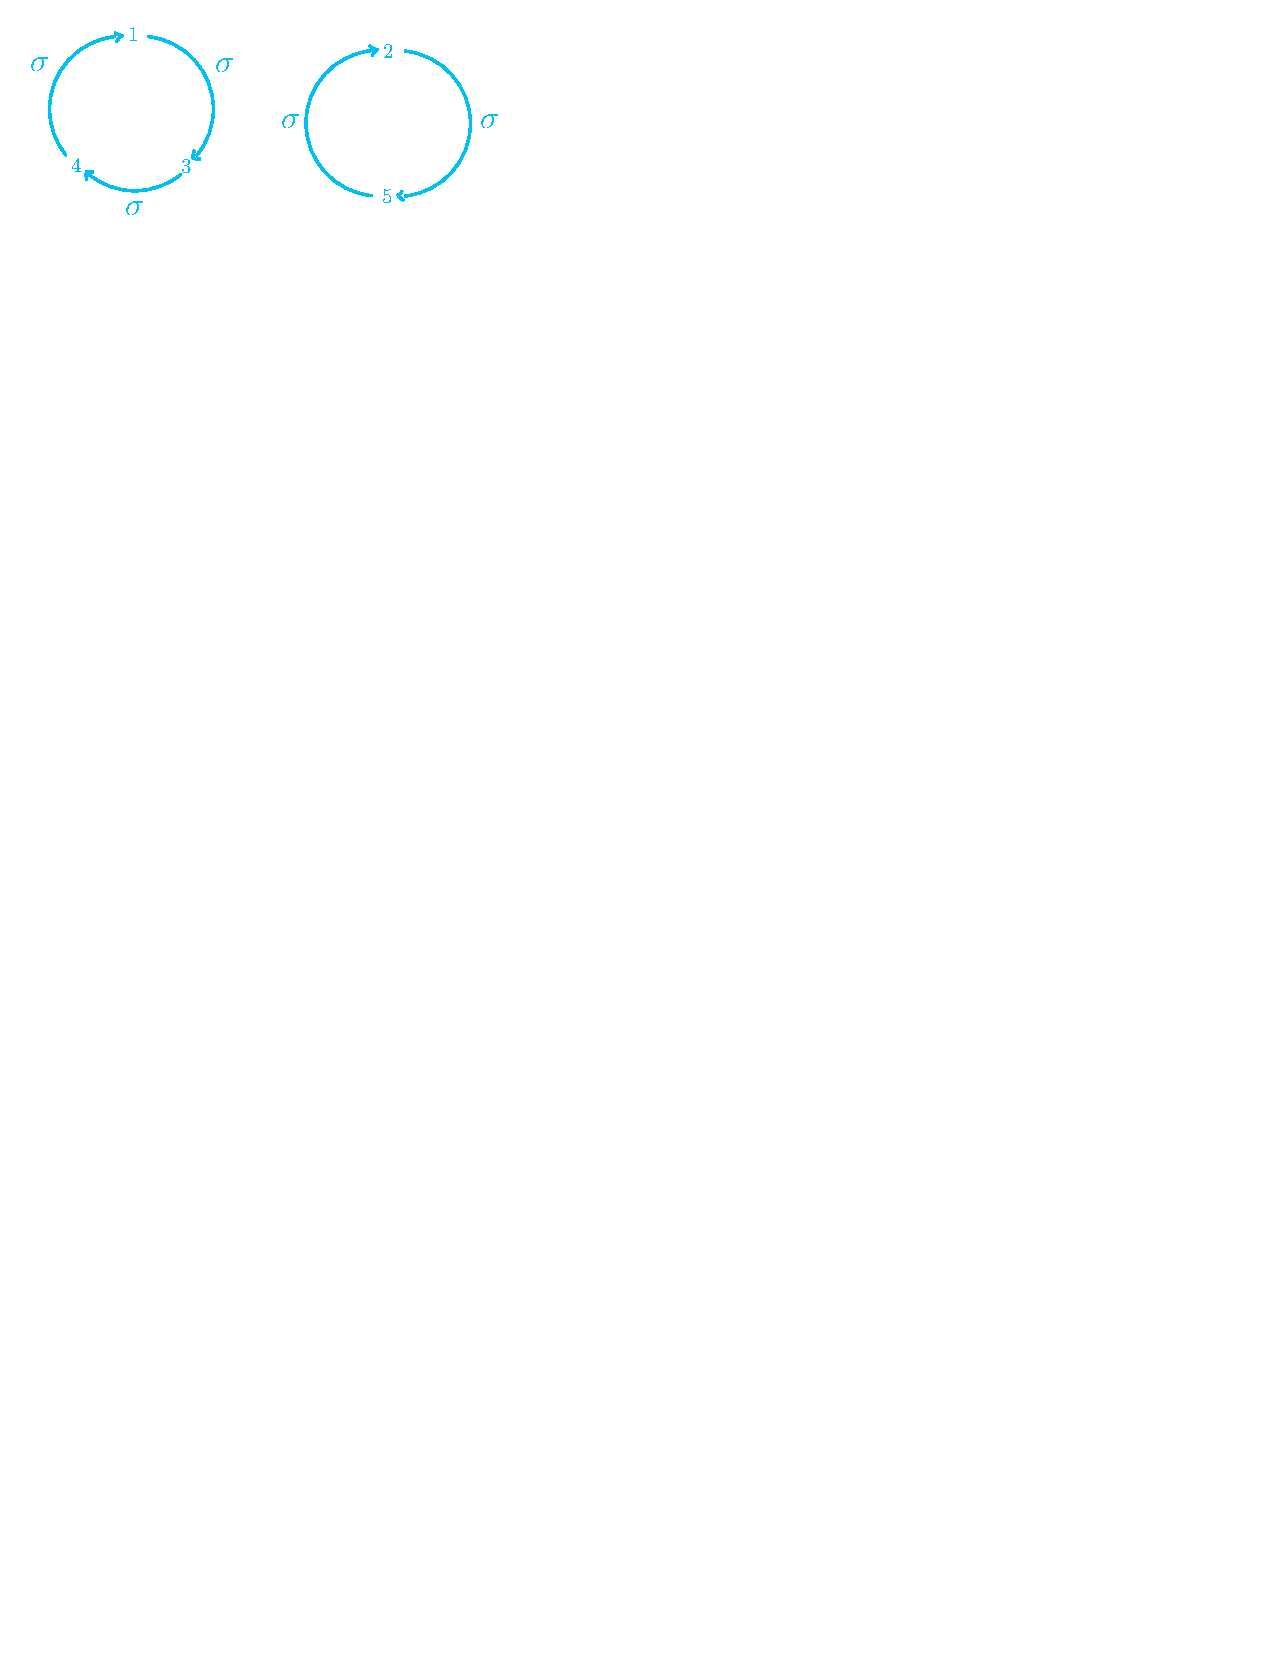
\includegraphics[width=0.8\textwidth, trim= 0.5cm 24cm 13cm 0.25cm,clip]{fig1.pdf}%LDRU
   \end{figure}
   \end{center}\pause
Entonces: 
$$\sg=35412=(134)(25).$$
\end{frame}

\begin{frame}[t]\frametitle{Un breve ejercicio}
Tome otra permutación de $5$ elementos, distinta a $\sg=35412$ y escríbala como:
\begin{itemize}
  \item Un emparejamiento.
  \item Una matriz.
  \item Una lista.
\end{itemize}
También:
\begin{itemize}
  \item Dibuje el gráfico de su permutación.
  \item Descompóngala por ciclos.
\end{itemize}
  
\end{frame}

\begin{frame}[t]\frametitle{El grupo simétrico}
  %Rápidamente:
  \begin{definition}
    El conjunto de todas las permutaciones es 
    $$S_n=\set{\sg\ \text{es una permutación de }\ [n]}.$$
  \end{definition}\pause
  \begin{example}
    En $S_2$: 
    $$S_2=\set{12,21}.$$
  \end{example}\pause 
  \begin{example}
    En $S_3$: 
    $$S_3=\set{123,213,132,321,231,312}.$$
  \end{example} 
\end{frame}

\begin{frame}[t]\frametitle{Estadísticas de permutaciones}
  %Rápidamente:
  \begin{definition}
    Una \underline{estadística} es una función: 
    $$f:\ S_n\to\bN.$$
  \end{definition}\pause
  \begin{itemize}[<+->]
    \item El \underline{orden} de una permutación es 
    $$\ord(\sg)=\min\set{n\in\bN\mid \sg^n=\text{id}}.$$
    \item El orden es una estadística: $\sg\mapsto\ord(\sg)$.
    \item Para $\sg=35412$, tenemos $\ord(\sg)=6$.
    \item De hecho 
    $$\ord(\sg)=\prod_{(\ast)}(\text{Longitudes de sus ciclos}).$$
  \end{itemize}
    
\end{frame}

\begin{frame}[t]\frametitle{Inversiones}
  \begin{definition}
    El \underline{número de inversiones} de una permutación $\sg$ es la cantidad de parejas $(\sg(i),\sg(j))$ con 
    $$i<j,\quad\text{y}\quad\sg(i)>\sg(j).$$
  \end{definition}\pause
  Para $\sg=35412$:\par
  \vspace{7em}\pause
  Es decir, $\inv(\sg)$ es una estadística.
\end{frame}

\begin{frame}[t]\frametitle{Descensos}
  \begin{definition}
    El \underline{número de descensos} de una permutación $\sg$ es la cantidad de índices $i$ con $\sg(i)>\sg(i+1)$.\par 
    El conjunto de descensos es $D(\sg)=\set{i\mid \sg(i)>\sg(i+1)}$
  \end{definition}\pause
  Para $\sg=35412$:\par
  \vspace{7em}\pause
  Nuevamente, $\des(\sg)$ es una estadística.
\end{frame}

\begin{frame}[t]\frametitle{Índice Mayor}
  \begin{definition}
    El \underline{índice mayor} de una permutación $\sg$ es la suma de los índices $i$ donde ocurren descensos.
  \end{definition}\pause
  Formalmente:
  $$\maj(\sg)=\sum_{i\in D(\sg)}i.$$\pause
  Para $\sg=35412$:
\end{frame}

\begin{frame}[t]\frametitle{Resumen y ejercicio}
  \begin{itemize}
    \itemsep=0.5em
    \item Órden: Cuantas veces la compongo para que sea la identidad.
    \item Inversiones: Número de parejas en \emph{orden opuesto}.
    \item Descensos: Número de inversiones \emph{seguidas}.
    \item Índice Mayor: Suma de los índices donde hay descensos.
  \end{itemize}\pause
  Con su permutación del inicio, encuentre el valor de las estadísticas.
\end{frame}

\begin{frame}[t]\frametitle{Contando con $q$'s}
\begin{example}
  Supongamos que tenemos 5 lápices, 2 botellas de agua y 3 cuadernos. Si al bulto echamos sólo uno de cada uno, ¿de cuántas maneras podemos acomodar el bulto?
\end{example}\pause 
\begin{example}
  Ahora dos lapices pesan 2 gramos, otros dos pesan 3 y uno 4. Los cuadernos pesan 10 y 12. Las botellas pesan 12, 12 y 13.\par 
  De las 30 maneras, cuantos arreglos van a pesar 25 gramos en total?
\end{example}

\end{frame}

\begin{frame}[t]\frametitle{$q$-análogos}
\begin{definition}
  Para un conjunto $X$ con una estadística $s: X\to\bN$, un \underline{$q$-análogo} de $|X|$ es 
  $$|X|_q=\sum_{x\in X} q^{s(x)}.$$
\end{definition}\pause 
Volviendo al ejemplo pasado\dots
$$L=2q^2+2q^3+q^4,\ C=q^{10}+q^{12},\ B=2q^{12}+q^{13}.$$\pause
Entonces 
$$L\cdot C\cdot B=q^{29} + 4 q^{28} + 7 q^{27} + 8 q^{26} + 6 q^{25} + 4 q^{24}.$$
\end{frame}


\begin{frame}[t]\frametitle{$q$-análogos para $S_3$}
  \begin{table}[]
    \begin{tabular}{llllll}\toprule
          &     & ord & inv & des & maj \\
          \midrule
    ()    & 123\ &     &     &     &     \\
    (12)  & 213\ &     &     &     &     \\
    (23)  & 132\ &     &     &     &     \\
    (13)  & 321\ &     &     &     &     \\
    (123) & 231\ &     &     &     &     \\
    (132) & 312\ &     &     &     &     \\
    \bottomrule
    \end{tabular}
    \end{table}\pause
  De aquí que 
  \begin{itemize}
    \itemsep=0.5em
    \item $\sum_{\sg\in S_3}q^{\ord(\sg)}=$
    \item $\sum_{\sg\in S_3}q^{\inv(\sg)}=$
    \item $\sum_{\sg\in S_3}q^{\des(\sg)}=$
    \item $\sum_{\sg\in S_3}q^{\maj(\sg)}=$
  \end{itemize}
\end{frame}

\begin{frame}[t]\frametitle{El factorial cuántico}
  Observemos que el resultado
  $$\sum_{\sg\in S_3}q^{\maj(\sg)}=\sum_{\sg\in S_3}q^{\inv(\sg)}$$
  se extiende a un hecho general:\pause
  \begin{theorem}
    Vale para todo $n$ que 
  $$\sum_{\sg\in S_n}q^{\maj(\sg)}=\sum_{\sg\in S_n}q^{\inv(\sg)}$$
y a esta cantidad le llamamos el \underline{factorial cuántico} $(n!)_q$.
  \end{theorem}
\end{frame}

\begin{frame}[t]\frametitle{El factorial cuántico}
  \begin{definition}
    El análogo cuántico de $n$ es 
    $$(n)_q=(1+q+q^2+\dots+q^{n-1})=\frac{q^n-1}{q-1}$$
  \end{definition}\pause
\begin{theorem}
  El factorial cuántico satisface la siguiente recurrencia:
  $$(n!)_q=(n)_q((n-1)!)_q.$$
\end{theorem}\pause 
Podemos extender mucho más y hablar del coeficiente binomial cuántico:
$$\binom{n}{k}_q=\frac{(n!)_q}{((n-k)!)_q(k!)_q}.$$
\end{frame}

\begin{frame}[t]\frametitle{¿Qué cuentan estos números?}
  Algunos objetos enumerados por números cuánticos:
  \begin{itemize}[<+->]
    \item Número de inversiones en $S_n$.
    \item En el plano proyectivo sobre $\bF_q$ con $q=p^k$ tenemos 
    $$|\bP^n_{\bF_q}|=(n+1)_q.$$
    \item El número de subespacios $k$ dimensionales de $\bF_q^n$ es $\binom{n}{k}_q$. 
  \end{itemize}\pause
  Y otros resultados interesantes como:\pause
  \begin{itemize}[<+->]
    \item El teorema binomial cuántico, si $xy=qyx$ entonces 
    $$(x+y)^n=\sum_{k=0}^{n}\binom{n}{k}_qx^k y^{n-k}.$$
    \item La recurrencia cuántica de Pascal:
    $$\binom{n}{k}_q=\binom{n-1}{k-1}_q+q^k\binom{n-1}{k}_q.$$
  \end{itemize}
\end{frame}

\begin{frame}[t]\frametitle{Otra, otra, otra\dots}
  Veamos una estadística más:
  \begin{definition}
    La \underline{carga} de una permutación $\sg$ se define de la siguiente manera:
    \begin{itemize}
      \item Escriba un subíndice de 0 bajo cada entrada de $\sg$.
      \item Para cada entrada $i>2$ aumente en 1 su subíndice si $i$ está a la derecha de $i-1$. Y sino, déjelo igual.
    \end{itemize}
    Sume todos los subíndices al final, eso es $c(\sg)$.
  \end{definition}\pause
  En el caso de $\sg=35412$ tenemos:\par
  \vspace{5em}\pause
  En general $\sum q^{c(g)}=(n!)_q$.
\end{frame}

  
\end{document}
